%%%%%%%%%%%%%%%%%%%%%%%%%%%%%% -*- Mode: Latex -*- %%%%%%%%%%%%%%%%%%%%%%%%%%%%
%% uhtest-abstract.tex -- 
%% Author          : Robert Brewer
%% Created On      : Fri Oct  2 16:30:18 1998
%% Last Modified By: Robert Brewer
%% Last Modified On: Fri Oct  2 16:30:25 1998
%% RCS: $Id: uhtest-abstract.tex,v 1.1 1998/10/06 02:06:30 rbrewer Exp $
%%%%%%%%%%%%%%%%%%%%%%%%%%%%%%%%%%%%%%%%%%%%%%%%%%%%%%%%%%%%%%%%%%%%%%%%%%%%%%%
%%   Copyright (C) 1998 Robert Brewer
%%%%%%%%%%%%%%%%%%%%%%%%%%%%%%%%%%%%%%%%%%%%%%%%%%%%%%%%%%%%%%%%%%%%%%%%%%%%%%%
%% 

%% Revision notes


\begin{abstract}
I propose an abstract distributed sensor network framework, Laha, that adaptively optimizes triggering, collection, detection, classification, sensor device power requirements, and bandwidth. The Laha data model can be conceptualized as a multilevel pyramid (see fig. \ref{laha-abstract-overview}). Laha Actors act on the data model to move data upward through the levels and to apply optimizations downward through the levels. 

The lowest level stores all recently received raw sensor data. This data expires and is automatically removed within a limited period of time (for example, 1 hour) unless the data is found to be interesting and is thus propagated upwards to the next level of the hierarchy.  Higher levels of the data hierarchy organize data in the same way, however each level adds context to the examined signal or signals. Context includes classifications, locality metrics, temporal metrics, or similarities to current or prior events. The highest level of the hierarchy, Phenomena, represents predictive capabilities of the sensor network which are then used to optimize and tune the lower levels.

A summary of the Laha abstract framework is provided as figure \ref{laha-abstract-overview}.


\begin{figure}
	\caption{Laha Conceptual Model Summary}
	\centering
	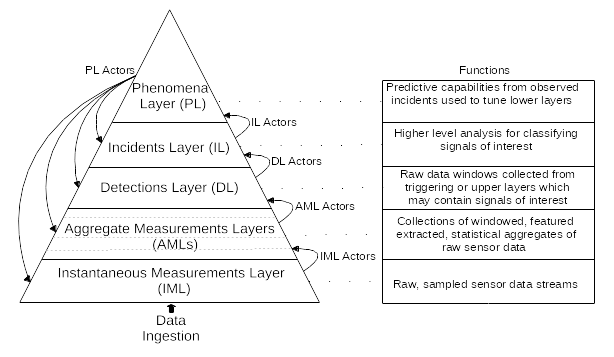
\includegraphics{figures/laha_abstract_overview.png}	
	\label{laha-abstract-overview}
\end{figure}
%Laha's data hierarchy includes the following levels. At each level, we further refine the data which is forwarded to higher layers in the hierarchy and filter out sensor noise. The lowest level, the Instantaneous Measurements Layer (IML) receives raw, sampled data from the network and forwards aggregate measurements to the Aggregate Measurements Layer (AML). The AML consumes feature extracted data streams to provide triggers for possible signals of interest which are forwarded to the Detections Layer (DL). The DL receives raw data from a subset of network sensors corresponding to time windows as determined in the AML. The DL data is forwarded to the Incidents Layer (IL) where standard and state of the art algorithms are used to identify and classify signals of interest within the windows provided by the DL. Finally, data from the DL is forwarded to the Phenomenon Layer (PL) where context, causality, and predictive analytics are created. Phenomena are then used to adaptively tune and optimize the lower levels of the hierarchy.

The Laha framework aims to provide seven useful benefits. Tiered management of Big Data where each tier has configurable time-to-live (TTL) requirements which relaxes bandwidth and storage requirements at the cost of potentially discarding important information. Automatically providing context to classified incidents based off of user and algorithmically tagged incidents. Adaptive optimization of triggering within the network to decrease bandwidth and increase accuracy. Adaptive optimizations for detection and classification algorithms power by Laha's Phenomena. Building of a model of the underlying sensor field topology by observing how signals travel and are received across multiple devices. Decreased bandwidth throughout the DSN as result of increased triggering, detection, and classification efficiency. Finally, minimizing of power sensor requirements as a result of increased triggering, detection, and classification efficiency. 

Laha will be evaluated by designing and implementing two Laha-compliant reference implementations OPQMauka and Lokahi. Open Power Quality (OPQ) is a power quality (PQ) network consisting of custom hardware and distributed software services that detect distributed PQ signals such as voltage sags and swells, frequency sags and swells, transients, THD, and other known PQ issues. OPQMauka is a distributed, plugin based middleware component of OPQ that performs higher level analysis, data management, and optimizations of the OPQ services. Lokahi is a distributed infrasound network consisting of mobile iOS and Android devices and multiple cloud based software services whose purpose is to supplement the International Monitoring System (IMS) in detecting large infrasound signals. 

The reference implementations will be deployed to test sites at UH Manoa and at the Infrasound Laboratory in Kailua-Kona, Big Island. 

Data collected from the PQ network will be validated against calibrated reference sensors that have already been installed at the power mains of a subset of buildings on campus. The Office of Energy Management at UH Manoa has given us full access to live and historic PQ data collected at these reference sensors. OPQBoxes will be co-located and placed in buildings with the reference sensors so that we can validate that the triggering and raw data streams we receive from the OPQBoxes are in line with what the reference sensors are observing. 

Data collected from the infrasound network will also be validated against industry standard calibrated BNK infrasound sensors. Further, signals in the infrasound network are known a priori since I am able to control the signals that are generated from our calibrated infrasound source, allowing further validation of received signals. 

To evaluate the seven benefits from Laha, several different approaches are taken depending on the Laha deployment. In the UH Manoa PQ deployment, we will co-locate sensors in our deployment and for each metric one of the sensors will use Laha's optimizations and the other sensor will not. This will provide metrics that allows us to compare and contrast our optimization techniques within the OPQ network. In the Lokahi infrasound network, we will run a series of experiments where we can produce the same infrasound signals in each experiment and only change the tuning and optimizations that Laha applies to generate metrics for evaluation within the Laha network.

% TODO provide name of industry standard OPQ sensors for validation
% TODO How do we evaluate the data?

I expect to deploy reference implementations before the end of 2018 with validated data collection beginning and continuing through Q3 2019. I anticipate writing my dissertation along side the deployment and data collection process and to be finished in Q3 2019. 

% Proposed contributions
\end{abstract}
